\documentclass{standalone}
\usepackage{tikz}
\begin{document}
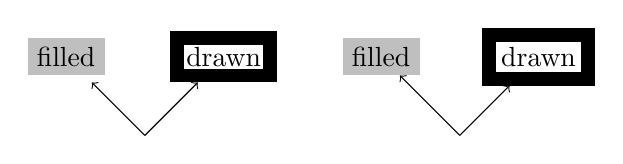
\begin{tikzpicture} 
\draw[line width=5pt] 
(0,0) node[fill=lightgray] (f1) {filled} 
(2,0) node[draw] (d1) {drawn}; 
\draw[->] (1,-1) -- (f1); 
\draw[->] (1,-1) -- (d1); 

\draw[line width=5pt] 
(4,0) node[outer sep=0pt,fill=lightgray] (f2) {filled} 
(6,0) node[inner sep=.5\pgflinewidth+2pt,draw] (d2) {drawn}; 
\draw[->] (5,-1) -- (f2); 
\draw[->] (5,-1) -- (d2); 
\end{tikzpicture}
\end{document}
